\documentclass[12pt]{article}
\usepackage[paperheight=210mm,paperwidth=148mm,top=2cm,bottom=2cm,left=1cm,right=1cm]{geometry}  % A5 paper
\usepackage{background}
\backgroundsetup{
    scale=1,
    opacity=0.1,
    angle=0,
    color=black,
    contents={%
        
\includegraphics[width=\paperwidth]{background}
    }
}
%%%%%%%%%%%%%%%%%%%%%%%%%%%%%%%%%%%%%%%%
\usepackage[utf8]{inputenc}
\usepackage[brazil]{babel}
\usepackage{titlesec}
%\usepackage[all]{hypcap}
\usepackage{multirow}
%\usepackage{tikz}
\usepackage{ctable}
%%%%%%%%%%%%%%%%%%%%%%%%%%%%%%%%%%%%%%%%
\renewcommand{\familydefault}{\sfdefault}
% \titleformat{\chapter}[display]
% {\bfseries\LARGE\sffamily}{\chaptertitlename}{10pt}{\LARGE}
% \titlespacing*{\chapter}{0pt}{10pt}{10pt}
% \numberwithin{table}{chapter}


\begin{document}
% Cover
\newgeometry{left=0cm, bottom=0cm, top=0cm, right=0cm}
\thispagestyle{empty}
\noindent  % To remove the unwanted white space.

\includegraphics{capa}
\NoBgThispage

\clearpage

\restoregeometry

\newpage

Olá,

no dia 16 de Maio de 2016 realizou-se o pré-evento para o SciPy Latin America
2016 no Centro de Informática e Automação do Estado de Santa Catarina S.A..
Foram mais de 6 horas de atividades nas quais os 13 participantes aprenderam um
pouco de Python, Git e LaTeX.
Agradecemos a ajuda de todos que estiveram envolvidos na realização do evento.

Att, \\
\indent Ivan Ogasawara \\
\indent Presidente da SciPy Latin America 2016


\newpage

\section*{Programa}

O programa divulgado para os participantes foi

% TODO Adicionar link para slides ou apresentação.
\begin{tabular}{cp{0.4\textwidth}l}
  \textbf{Horário} & \textbf{Título} & \textbf{Instrutor} \\
  9h-10h & SciTools Install Fest: Python - Anaconda, LaTeX, Git & \\
  10h10-12h10 & Introdução ao Python & Mário Sergio \\
  12h10-13h40 & Almoço \\
  13h40-14h40 & LaTeX - Automatizando a criação de PDFs com LaTeX+Python & Melissa Mendonça \\
  14h50-15h50 & Git/GitHub & Matheus Magrin \\
  16h00-17h00 & Open Science / Ciência Aberta & Ivan Ogassavara \\
\end{tabular}

\begin{figure}[!htb]
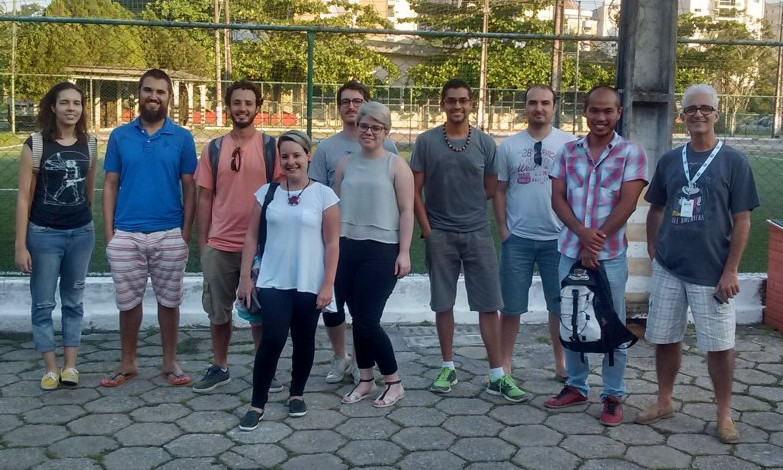
\includegraphics[width=\textwidth]{../../media/photos/pre4-cut}
\caption{Participantes ao final do evento}
\end{figure}

Esse cronograma foi parcialmente cumprido.

No período da manhã as atividades ocorreram dentro do horário previsto, porém muitos dos participantes
não chegaram no horário agendado. Como a primeira atividade era a instalação de
softwares o atraso dos participantes não comprometeu as demais atividades que se
sucediam.

A programação inicial não levou em consideração a complexidade do Git.
Deveria ter sido deixado um período de ao menos 2 horas para esta atividade.
O horário da última atividade foi cedido para dar continuidade com a sessão de
Git. Infelizmente, mesmo com o tempo adicional não foi possível cobrir todo o
conteúdo programado. Os participantes foram convidados à participar do tutorial
de Git que ocorrerá no SciPy Latin America 2016.

\newpage

\section*{Público}

Entre os dias 8 de Abril e 16 de Abril (quando o evento foi realizado)
tivemos 29 inscritos (26 homens e 3 mulheres) dos quais apenas 13 apareceram no
dia (8 homens e 5 mulheres).

\begin{figure}[!htb]
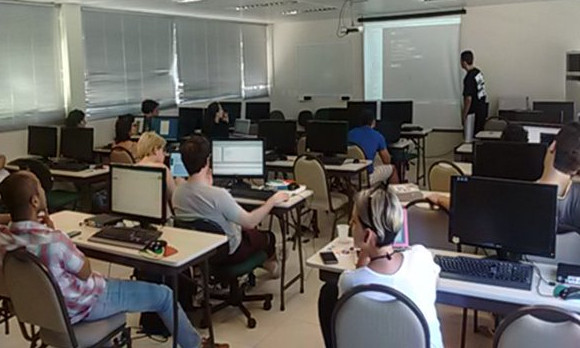
\includegraphics[width=\textwidth]{../../media/photos/pre0-cut}
\caption{Participantes}
\end{figure}

Esperávamos em torno de 50\% de presença tendo em vista que não cobramos
inscrição dos participantes.
Algumas pessoas que não tinham feito inscrição antecipada apareceram e puderam
participar do evento.

A divulgação do evento foi realizada durante apenas uma semana.
Ter um período de divulgação poderia ter aumentado o número de participantes.
Outro fator que pode ter influenciado o baixo número de participantes é que no
mesmo dia foi realizado a prova de proficiência na língua inglesa
(TOEFL) na UFSC e muitos interessados iriam realizar esse exame.
\newpage

\section*{Repercussão}

Infelizmente nossa equipe só publicou 4 tweets durante o evento que foram
apreciadas ou repetidas por algumas poucas pessoas.
A pessoa a cargo da cobertura do evento nas redes sociais era novata nessa área
e acabou publicando os tweets na conta pessoal e não na conta do SciPy Latin
America de forma que os tweets não foram publicados na página da comunidade no
Facebook.

Alguns dos participantes manifestaram interesse em montar um grupo de estudo de Python. Ivan
Ogasawara já está cuidando de um grupo de estudo na Universidade Federal de Santa Catarina e
convidou os interessados à participarem do grupo.

Após a realização do evento, foi enviado aos participantes um questionário para recebermos suas
opiniões sobre as palestras e o evento.

\begin{figure}[!h]
    \centering
    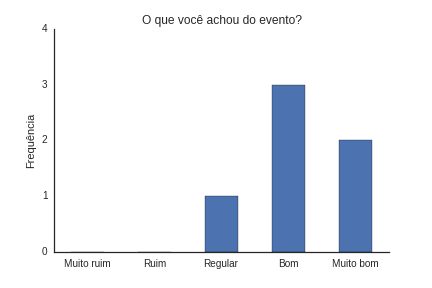
\includegraphics[height=0.25\textheight]{images/evento1.png}
\end{figure}

No geral o evento foi satisfatório de acordo com os participantes
(informações sobre cada atividade são fornecidas no final desse relatório).

\newpage

\section*{Finanças}

As despesas para o evento foram

\begin{tabular}{p{0.6\textwidth}r}
  \textbf{Descrição} & \textbf{Valor} (em R\$) \\\hline
  Locação do espaço & 600,00 \\
  Transporte\footnotemark & 400,00 \\
  Almoço\footnotemark  & 200,00 \\\hline
  \textbf{Total} & 1200,00
\end{tabular}
\setcounter{footnote}{1}
\footnotetext{R\$40,00 por trajeto para cada instrutor mais funcionário do Centro de Informática e Automação do Estado de Santa Catarina S.A.}
\addtocounter{footnote}{1}
\footnotetext{R\$40,00 para cada instrutor mais funcionário do Centro de Informática e Automação do Estado de Santa Catarina S.A.}

As despesas foram cobertas pelo Centro de Informática e Automação do Estado de Santa Catarina
S.A. e instrutores.

\newpage

\section*{Repostas do questionário de satisfação (Python)}

\begin{center}
    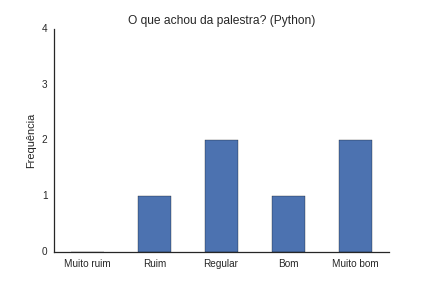
\includegraphics[height=0.25\textheight]{images/python1.png}
\end{center}

\begin{center}
    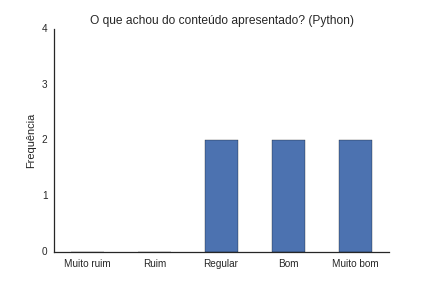
\includegraphics[height=0.25\textheight]{images/python2.png}
\end{center}

\begin{center}
    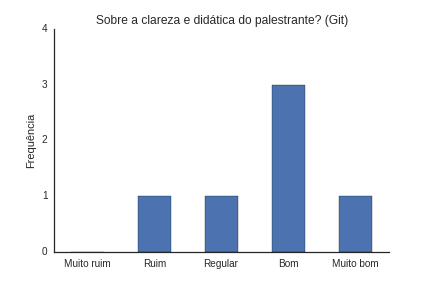
\includegraphics[height=0.25\textheight]{images/python3.png}
\end{center}

\section*{Repostas do questionário de satisfação (LaTeX)}

\begin{center}
    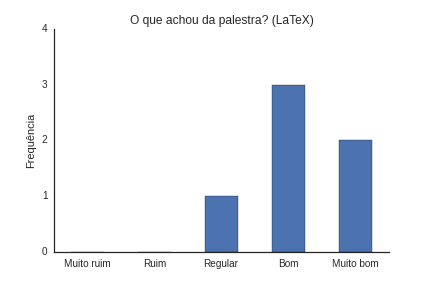
\includegraphics[height=0.25\textheight]{images/latex1.png}
\end{center}

\begin{center}
    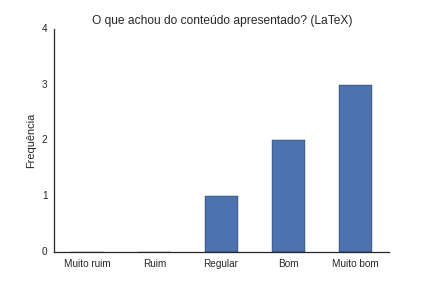
\includegraphics[height=0.25\textheight]{images/latex2.png}
\end{center}

\begin{center}
    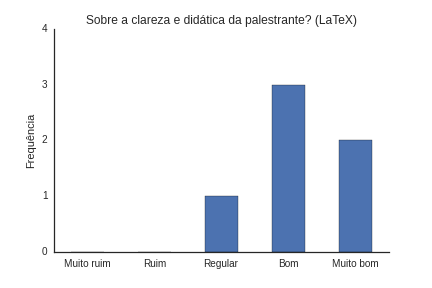
\includegraphics[height=0.25\textheight]{images/latex3.png}
\end{center}

\section*{Repostas do questionário de satisfação (Git)}

\begin{center}
    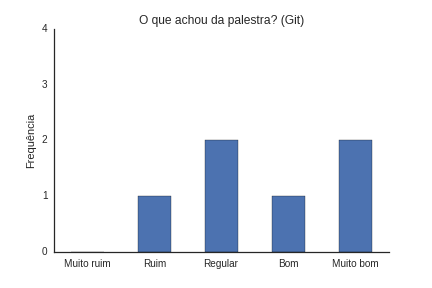
\includegraphics[height=0.25\textheight]{images/git1.png}
\end{center}

\begin{center}
    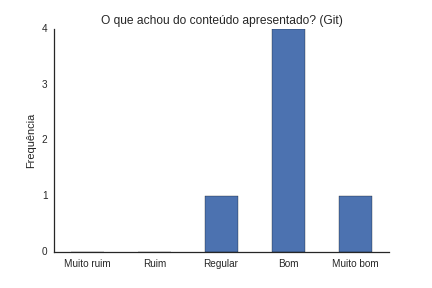
\includegraphics[height=0.25\textheight]{images/git2.png}
\end{center}

\begin{center}
    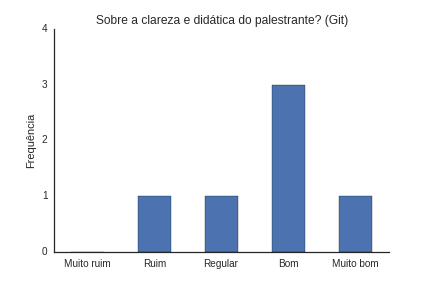
\includegraphics[height=0.25\textheight]{images/git3.png}
\end{center}


\end{document}
